\documentclass{article}
\usepackage[cm]{fullpage}
\usepackage{parskip}
\usepackage[usenames,dvipsnames,svgnames,table]{xcolor} % Provides more color options
\usepackage[bookmarks,colorlinks,linktoc=all,linkcolor=DarkGreen,urlcolor=Blue]{hyperref}
\usepackage{graphicx}
\usepackage[symbol]{footmisc}
\title{FPGA Block Diagram}
\author{Matt Kline, James Gordon, Tyler Kuske, and Creighton Long}
\pagenumbering{gobble}
\begin{document}
\maketitle

\begin{center}
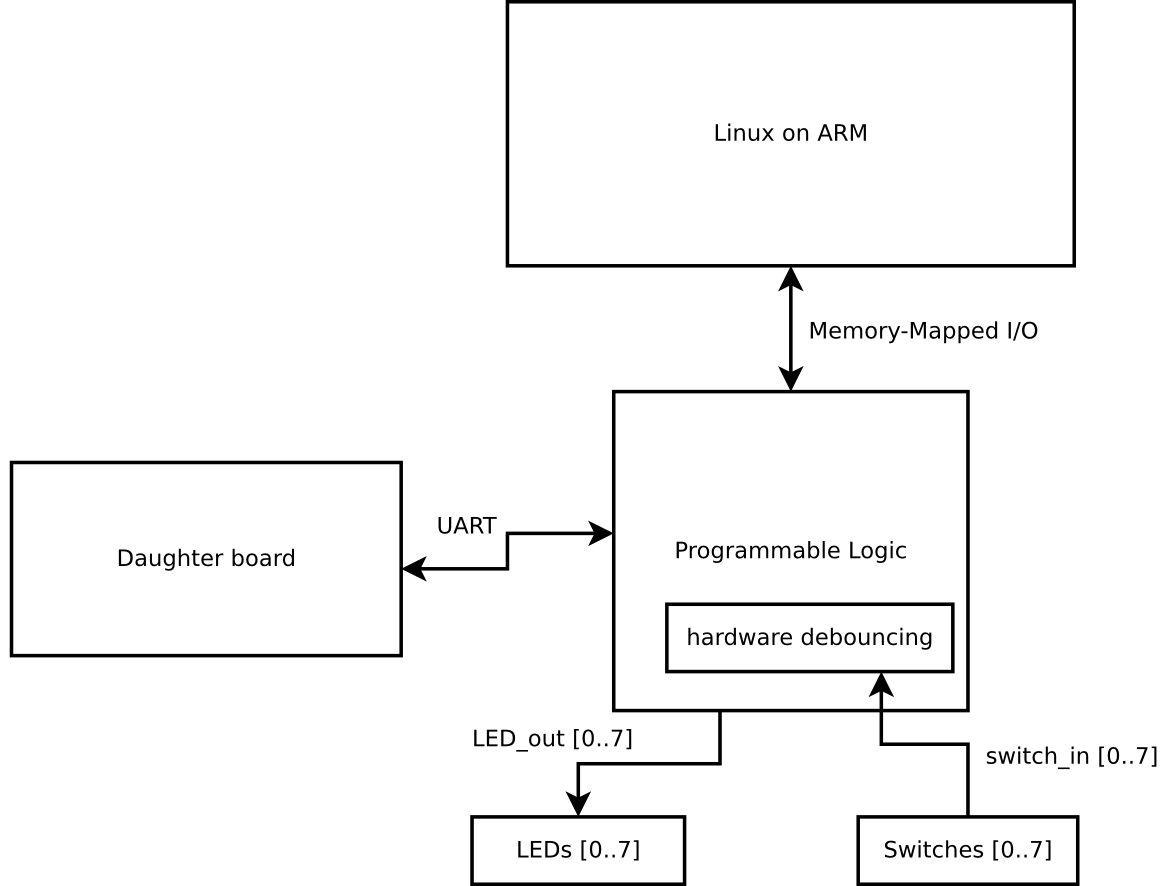
\includegraphics[height=0.4\textheight, keepaspectratio]{fpga_block.png}
\end{center}

\vspace{2cm}

Our FPGA plans are simple by design. Because our daughter board, our targets,
and our guns will all have their microcontroller, the work can be done in software.
This is advantageous as software should be easier to debug and does not have to be respun if plans change.
The ZedBoard switches can be used for basic configuration, and will be debounced in-hardware by programmable logic.
Besides that, the FPGA will serve simply as a routing layer, routing the LEDs to a memory-mapped register
and routing the UART communication from the daughter board.
UART was chosen for the daughter board because it can be directly debugged by another machine and provides
an extremely simple interface.
Speed should not be a concern, as the data we will be passing across the link is relatively small.

\end{document}
